% \documentclass[pdflatex,11pt]{aghdpl}
% \documentclass{aghdpl}               % przy kompilacji programem latex
\documentclass[pdflatex,en]{aghdpl}  % praca w języku angielskim
\usepackage[british,UKenglish,USenglish,english]{babel}
\usepackage[utf8]{inputenc}

\usepackage[backend=bibtex,
%style=numeric,
bibencoding=ascii,
style=alphabetic
%style=reading
]{biblatex}

\addbibresource{bibliografia.bib}

% dodatkowe pakiety
\usepackage{enumerate}
\usepackage{listings}
\usepackage{float}
\usepackage{siunitx}

\lstloadlanguages{TeX}

\lstset{
  literate={ą}{{\k{a}}}1
           {ć}{{\'c}}1
           {ę}{{\k{e}}}1
           {ó}{{\'o}}1
           {ń}{{\'n}}1
           {ł}{{\l{}}}1
           {ś}{{\'s}}1
           {ź}{{\'z}}1
           {ż}{{\.z}}1
           {Ą}{{\k{A}}}1
           {Ć}{{\'C}}1
           {Ę}{{\k{E}}}1
           {Ó}{{\'O}}1
           {Ń}{{\'N}}1
           {Ł}{{\L{}}}1
           {Ś}{{\'S}}1
           {Ź}{{\'Z}}1
           {Ż}{{\.Z}}1
}

%---------------------------------------------------------------------------

\author{Grzegorz Gajoch}
\shortauthor{G. Gajoch}

\titlePL{Budowa sensora pochłoniętej dawki promieniowania jonizującego (TID) dla pico-satelitów typu CubeSat}
\titleEN{Total Ionizing Dose (TID) sensor for CubeSat~pico-satellites}

\shorttitlePL{Budowa sensora pochłoniętej dawki promieniowania jonizującego (TID) dla pico-satelitów typu CubeSat} % skrócona wersja tytułu jeśli jest bardzo długi
\shorttitleEN{Total Ionizing Dose (TID) sensor for CubeSat~pico-satellites}

\thesistypePL{Praca inżynierksa}
\thesistypeEN{Bachelor of Science Thesis}

\supervisorPL{dr inż. Cerazy Worek}
\supervisorEN{Cerazy Worek Ph.D}

\date{2016}

\departmentPL{Katedra Elektroniki}
\departmentEN{Department of Electronics}

\facultyPL{Wydział Informatyki, Elektroniki i Telekomunikacji}
\facultyEN{Faculty of Computer Science, Electronics and Telecommunications}

\acknowledgements{Serdecznie dziękuję \dots tu ciąg dalszych podziękowań np. dla promotora, żony, sąsiada itp.}


%---------------------------------------------------------------------------

\begin{document}

\titlepages

\tableofcontents
\clearpage

\chapter{Principles}

\section{Space radiation effects on electronics}
In space electronics design there are two major radiation effects to be considered. Each has different background and different mitigation schemes.

\subsection{Single Event Effects}
Single Event Effects are connected with very high energy particles striking electronic component. Is can cause different problems:


Major mitigation scheme is to 
\subsection{Total Ionising Dose}


\section{Need for TID radiation measurements}
    As mentioned before, TID can be very dangerous - ionising radiation accumulated can cause any device to stop functioning. Therefore, devices have to be tested for amount of radiation they can withstand ("radiation tests"). The radiation flux on orbit is well-described, but the TID accumulated during mission should be monitored to be able to abort and utilise sattelite before its fail. 

\section{PW-Sat2 mission}
    PW-Sat2 is Polish second student satellite, mainly build by students from Warsaw Univeristy of Technology. The cooperation between author and PW-Sat2 team led to this thesis.
    
\subsection{Main purpose}
    Main goal of PW-Sat2 is to test deorbitation sail mechanism. The sail (2x2 m size) will open from the back of the satellite and cause the orbit to decay faster.
    
    % photo 
\subsection{Orbit \& lifetime}
    PW-Sat2 mission is planned to last for 40 days. After 40 days sail will be opened and satellite will deorbit in couple of weeks time.
    
    PW-Sat2 will be launched on top of Falon9 rocket from SpaceX company, planned Q4 2017. The final orbit is 565 km sun-synchronous orbit.
    
    
\subsection{Radiation analysis}
    To estimate radiation dose accumulated by PW-Sat2 the simulation in SPENVIS envirnoment was performed. 
    % radiation patterns
    On orbit there are clearly seen Van-Allen radiation belts and South Atlantic Anomaly. 
    
    The total dose accumulated by satellite on this orbit is about $N rad$.
\chapter{Design requirements}

In this chapter the requirement for the TID sensor will be presented.

Sensor is designed to be flown on-board of PW-Sat2 satellite. Therefore it should be designed for its particular requirements. In addition, it should be designed having in mind active space standard and launcher requirements.


\section{PW-Sat2 mission}
	Presented sensor is scheduled to be launched on PW-Sat2 satellite \cite{PW-Sat2URL}. Therefore it should be designed especially for this particular type of mission. In this section PW-Sat2 mission will be presented. On fig. \ref{PW-Sat_render_01} exploded render is presented.
	
	\begin{figure}[h]
		\centering
		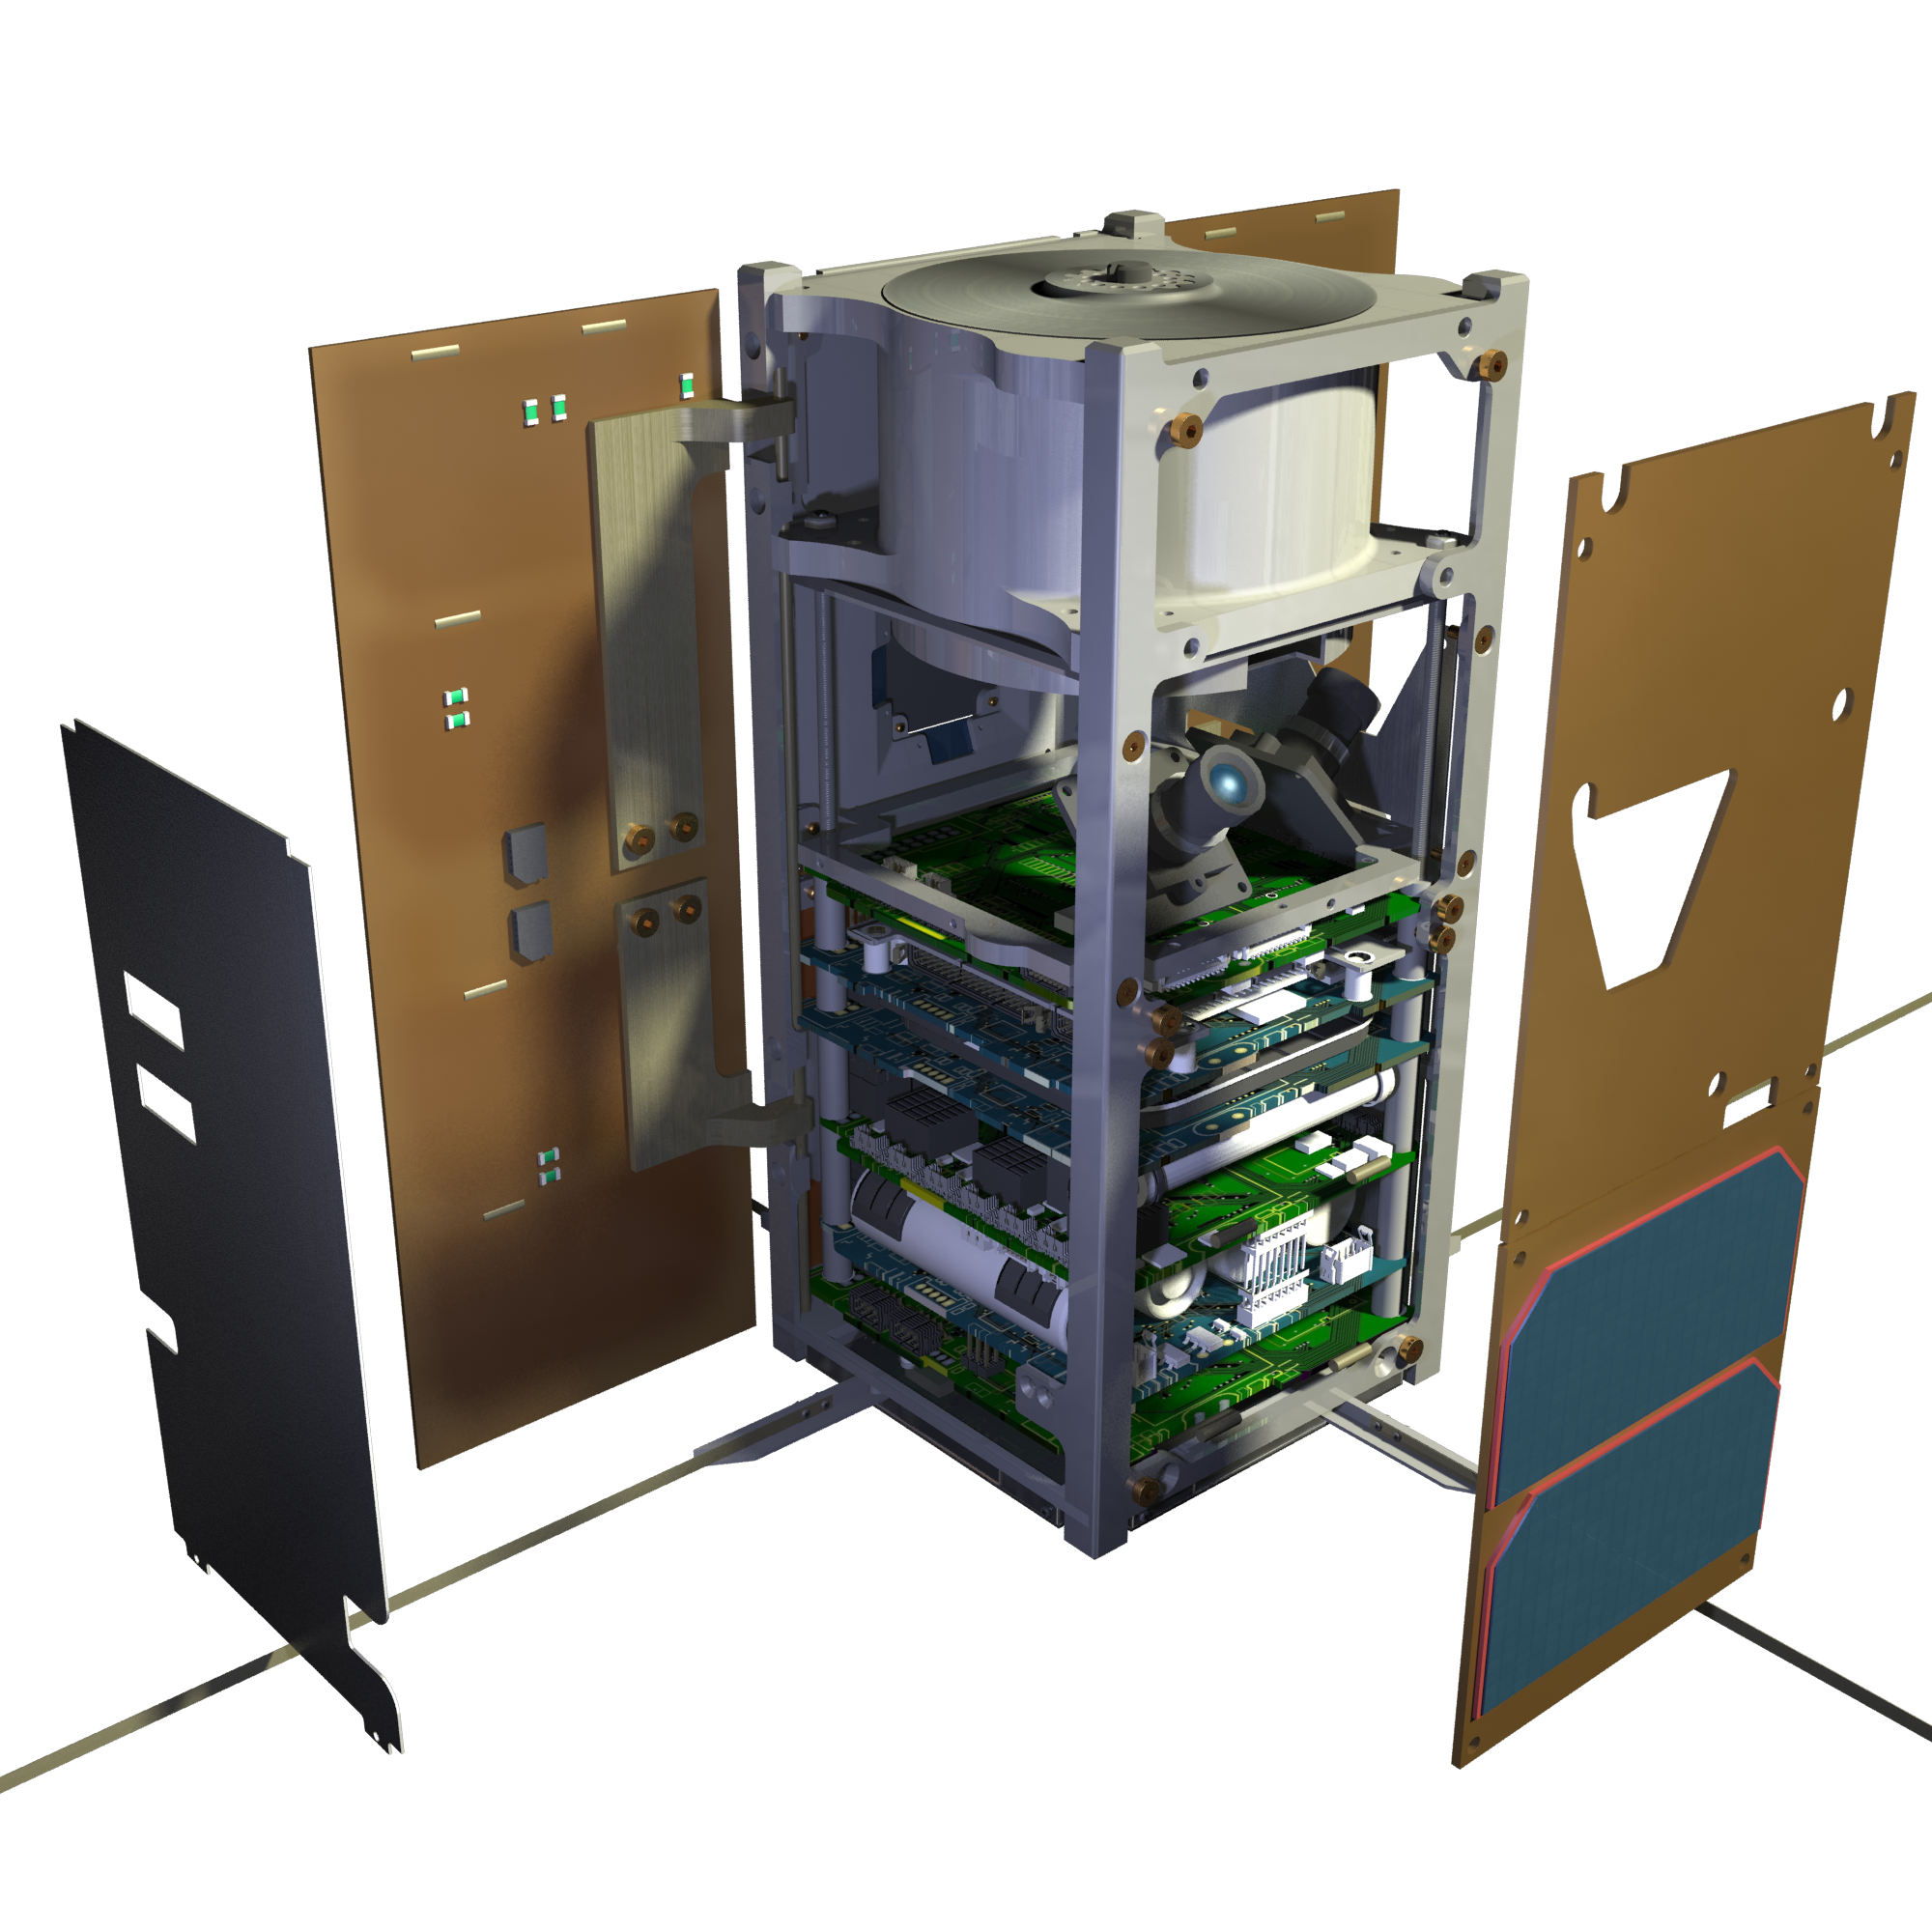
\includegraphics[width=0.5\paperwidth]{img/PW-Sat2_render_01.png}
		\caption{PW-Sat2 render (by M. Świetlik)}
		\label{PW-Sat_render_01}
	\end{figure}

	PW-Sat2 is scheduled to be launched on Falon9 rocket from SpaceX company in Q4 2017.
	
	\begin{figure}[H]
		\centering
		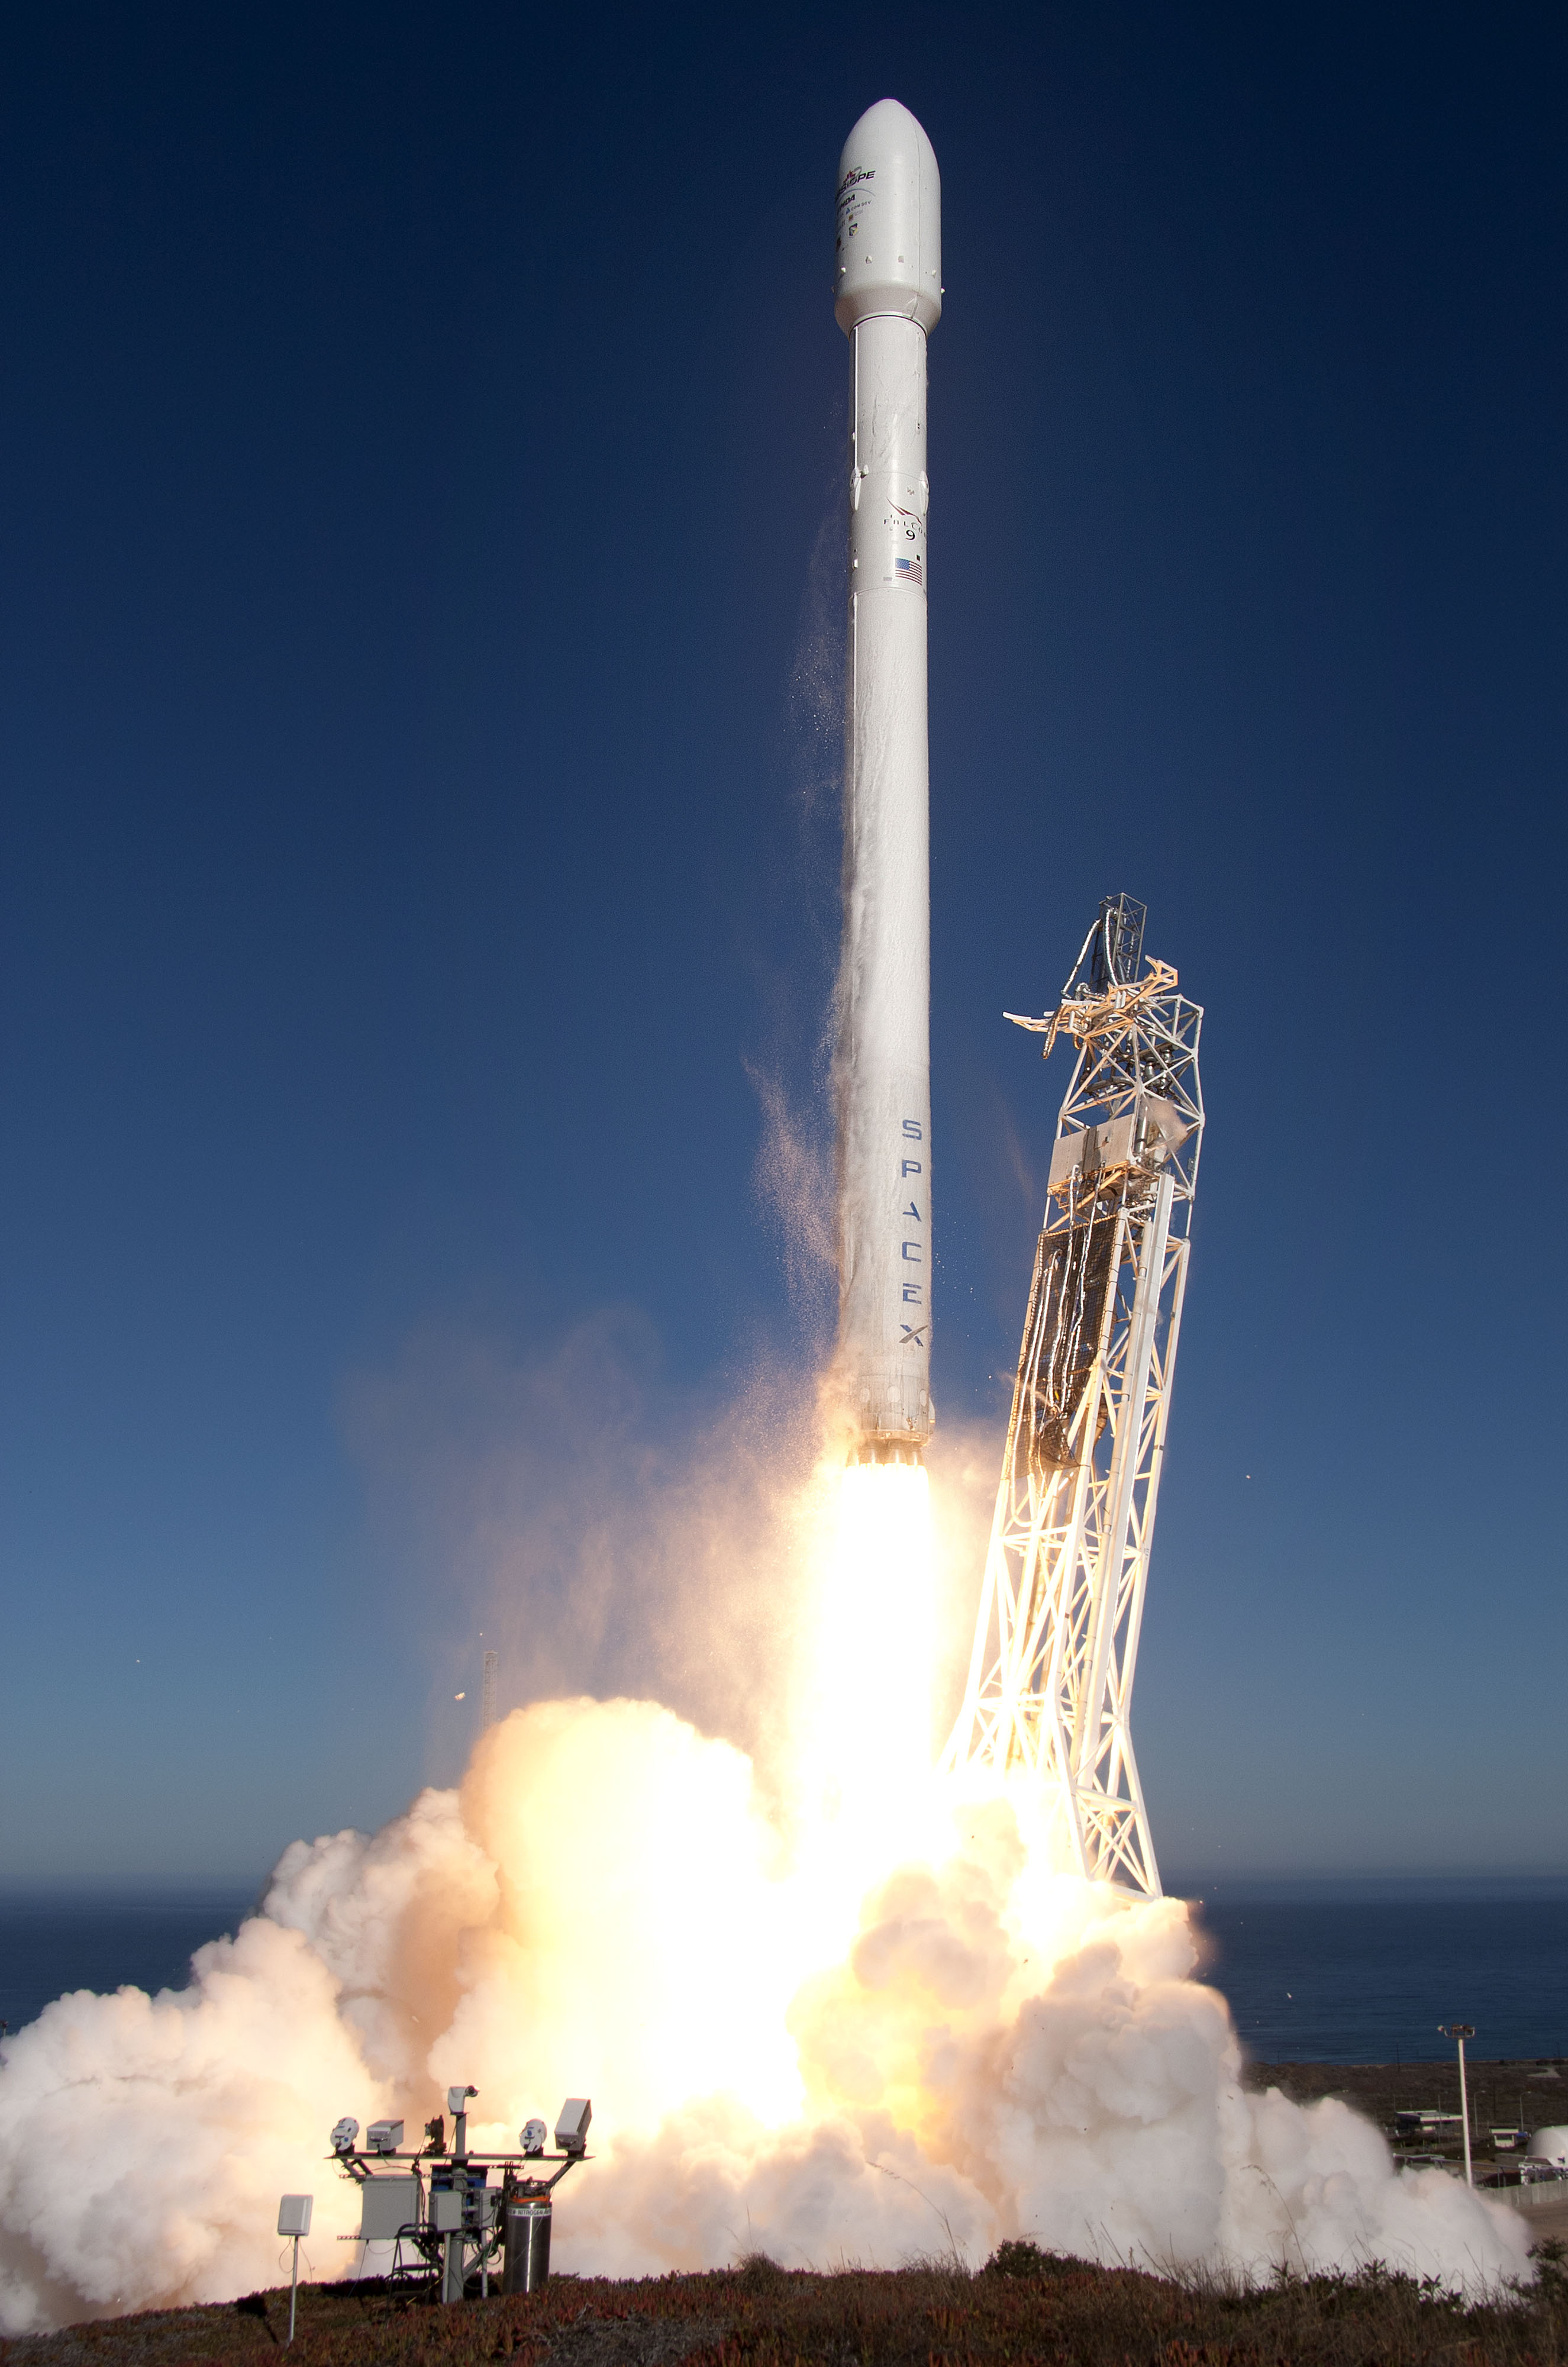
\includegraphics[width=0.3\paperwidth]{img/Falcon9.jpg}
		\caption{Falcon9 rocket. Source: \url{www.spacex.com}}
		\label{PW-Sat_render_01}
	\end{figure}
	
	
\subsection{Primary mission}
	Primary mission of PW-Sat2 is to test deorbiting sail. Its purpose is to increase atmospheric drag and shorten satellite life. This method of deorbitation could be easy way to reduce space debris on LEO. Render of PW-Sat2 with opened sail is on \ref{PW-Sat_render_sail}.
	
	\begin{figure}[H]
		\centering
		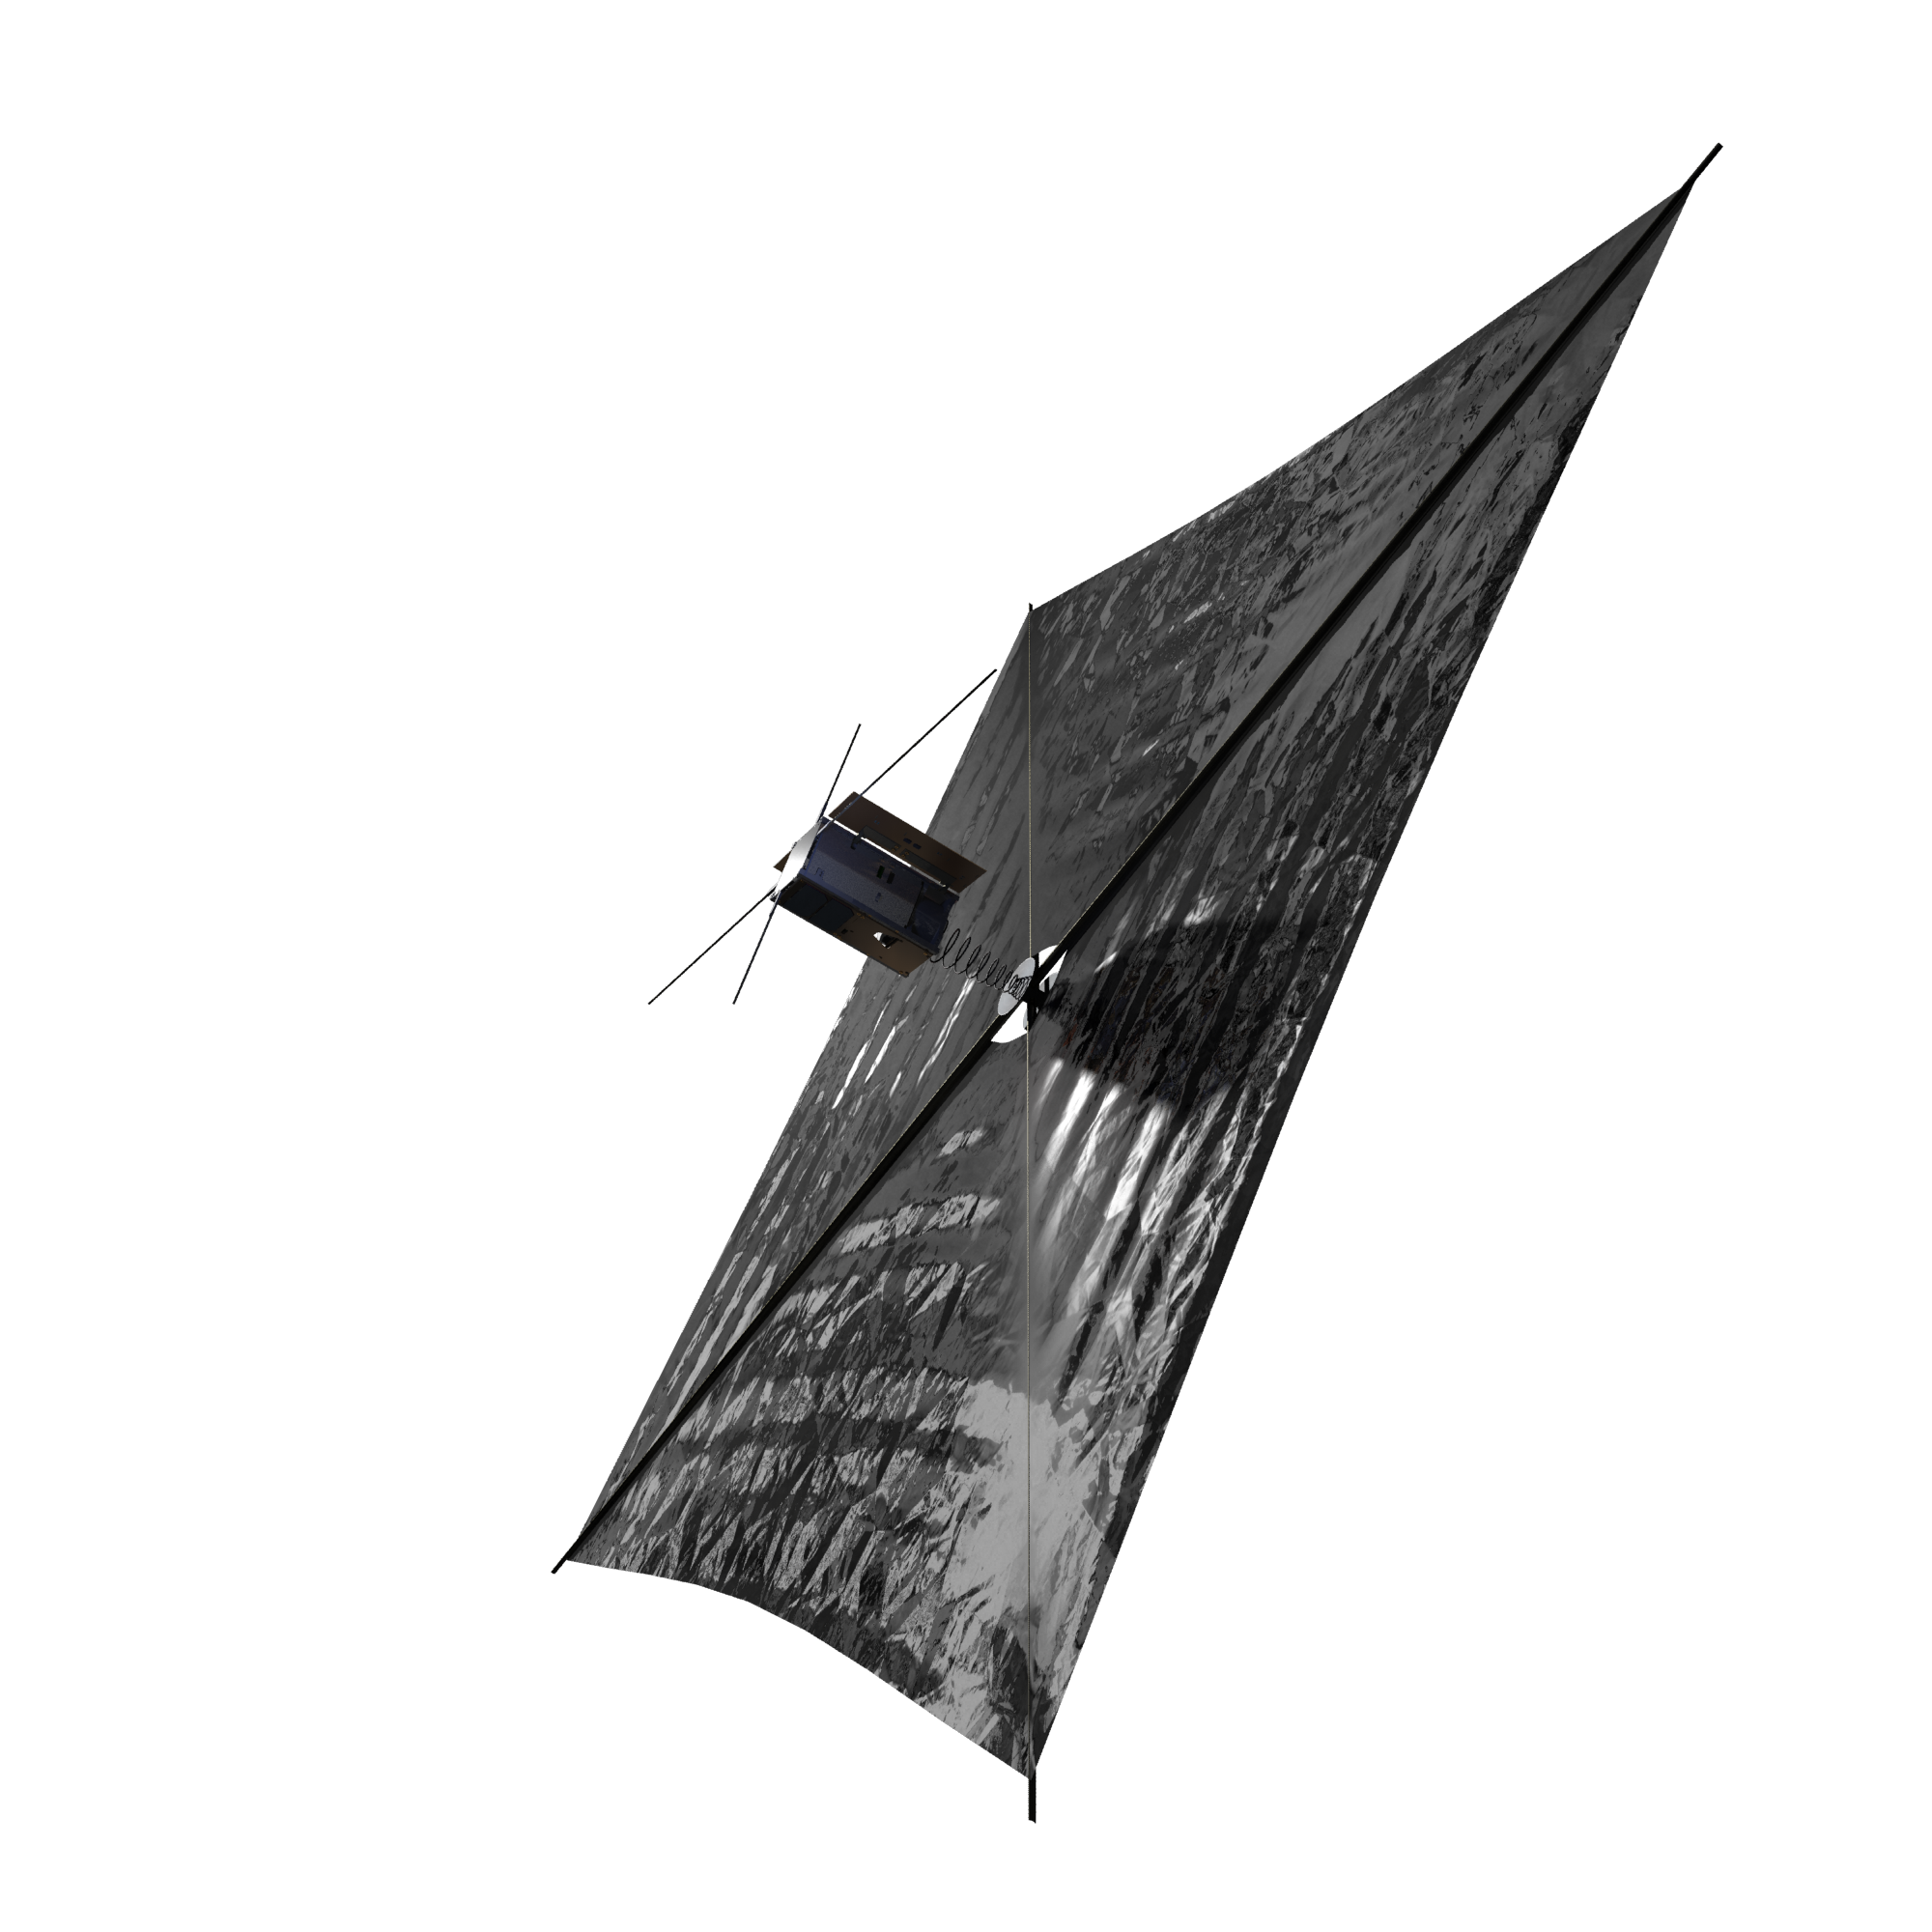
\includegraphics[width=0.7\paperwidth]{img/PW-Sat2_render_02.png}
		\caption{PW-Sat2 with opened sail (by M. Świetlik)}
		\label{PW-Sat_render_sail}
	\end{figure}
	
	More information can be found in \cite{DDC_article}.
	
\subsection{Lifetime}
	Due to its primary mission PW-Sat2 mission is planned to be 40 days long. After this time deorbit sail will open, possibly causing lack of communication with satellite. Therefore sensor should be able to measure dose absorbed during 40 days on orbit.
	
\subsection{Orbit}
	PW-Sat2 in planned to be launched to sun-synchronous circular orbit of attitude $575~km$, with LTAN of $10:30$ \cite{PWSAT_MA_CDR}.
	

\subsection{Radiation analysis}
	Simulations in SPENVIS \cite{SPENVIS_URL} were performed to determine TID accumulated during PW-Sat2 mission. On fig \ref{TIDvsSheilding} dose as a function of shielding thickness was plotted.

	\begin{figure}[H]
		\centering
		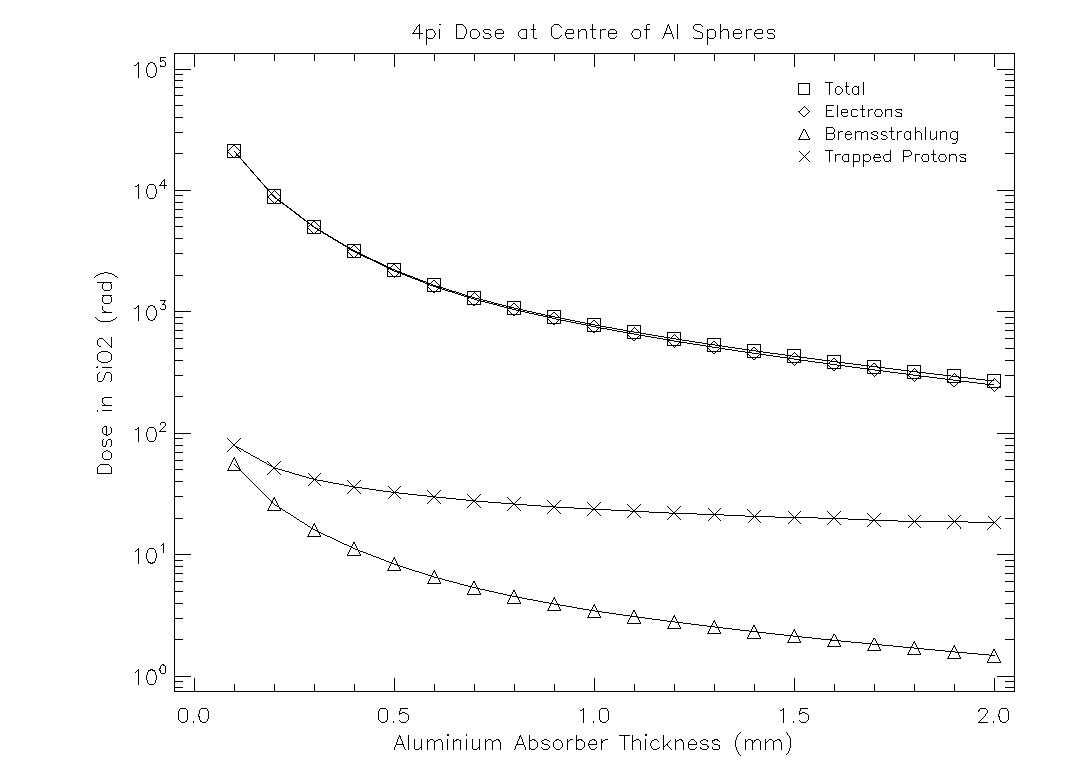
\includegraphics[width=0.7\paperwidth]{img/dose.eps}
		\caption{TID vs shielding}
		\label{TIDvsSheilding}
	\end{figure}

	Shielding of PW-Sat2 is about $1~mm$ thick (aluminium sides as well as aluminium base for solar cells - \ref{PW-Sat_render_01}). Therefore predicted dose during PW-Sat2 mission is about $1$~kRad.


\section{Sensor requirements}
	In this section sensor requirements are presented.

\subsection{Range}
	Total range of the sensor should be more than predicted dose ($>~1$~kRad). With $300\%$ reserve: designed sensor should have range of more than $3$~kRad.
	
\subsection{Accuracy \& resolution}
	Sensor should be able to detect low radiation doses. Its resolution should be lower than $0.1$~kRad, with accuracy of less than $0.5$~kRad.


\section{Electrical requirements}
	
\subsection{Electronics stack}
\subsection{Power}
\subsection{Data interface}
\subsection{Radiation immunity}
\subsection{Reliability of components}

\section{Mechanical requirements}
\subsection{PCB stack \& PCB restrictions}
\subsection{Space available}
\subsection{Vibration}
\subsection{Operation temperature}
\subsection{Thermal cycles}

\section{Applicable standards}


% 1. Introduction
% 
% 2. Terms, definitions and abbreviated terms 
% 2.1. Abbreviated terms
% 2.2. Conventions
% 
% 3. Principles
% 3.1. Space radiation effects on electronics
% 3.1.1. Single Events Effects
% 3.1.2. Total Ionising Dose
% 3.2. Need for TID radiation measurements
% 
% 
% 
% 
% 4. Design requirements
% 4.1. Sensor requirements
% 4.1.2. Required sensitivity
% 4.1.3. Required accuracy
% 4.2. Applicable standards
%
% 4.3. PW-Sat2 mission
% 4.3.1. Main purpose
% 4.3.2. Orbit \& lifetime
% 4.3.3. Radiation analysis
%
% 4.3. Electrical requirements
% 4.3.1. Electronics stack
% 4.3.2. Power
% 4.3.3. Data interface
% 4.3.4. Radiation immunity
% 4.3.5. Reliability of components
%
% 4.4. Mechanical requirements
% 4.4.1. PCB stack \& PCB restrictions
% 4.4.2. Space available
% 4.4.3. Vibration
% 4.4.4. Operation temperature
% 4.4.5. Thermal cycles
% 
% 
% 5. Sensor design
% 5.1. TID measurement technique
% 5.2.1. Accumulating particles in MOSFET
% 5.2.2. Physical phenomena background
% 
% 5.3. Tradeoff analysis
% 5.3.1. Measurement channels
% 5.3.2. Measurement accuracy
% 
% 5.3. Block diagram
% 
% 5.4. Components selection
% 5.4.1. MOSFET
% 5.4.2. ADC
% 5.4.3. Microcontroller
% 5.4.4. Passives
% 
% 5.5. Die temperature measurement
% 5.5.1. Build-in ESD diode
% 5.5.2. Body diode
% 5.6. Bias of MOSFET gate
% 
% 6. Sensor implementation
% 6.1. Analog front-end
% 6.1.1. Current source
% 6.1.2. Threshold voltage readout
% 6.1.3. Temperature measurement
% 6.2. Digital
% 6.2.1. Microcontroller
% 6.2.2. ADC
% 6.2.3. OBC interface
% 6.3. Software design
% 6.3.1. Other tasks running on the same processor
% 6.3.2. AVR-HAL
% 6.3.3. I2C-slave module
% 6.3.4. Measurement algorithm
% 
% 7. Sensor prototypes
% 7.1. Calibration prototype v0.1
% 7.2. Calibration prototype v0.2
% 7.3. TID Sensor prototype board
% 
% 8. Sensor production
% 8.1. Payload board
% 8.1.1. PCB layout 
% 8.1.2. 3D model
% 8.2. PCB production
% 8.3. Component soldering
% 
% 9. Sensor tests
% 9.1. Measurement noise
% 9.2. Temperature stability
% 9.3. Operational temprature
% 9.4. Radiation tests
% 9.5. Estimated lifetime on different orbits
% 9.6. Digital interfaces
% 
% 10. Summary
% 
% Figures
% Tables



% itd.
% \appendix
% \include{dodatekA}
% \include{dodatekB}
% itd.

\printbibliography

\end{document}
